\documentclass[12pt]{article}
\usepackage[left=15mm,top=0.5in,bottom=0.5in,centering]{geometry}
\usepackage{listings}
\usepackage{framed}
\usepackage{graphicx}
\usepackage{wrapfig}
\usepackage{floatrow}
\usepackage{subfigure}
\usepackage{color}
\usepackage{amsmath}
\usepackage{lipsum}
\usepackage{hyperref}
\usepackage{amssymb}
\usepackage{rotating}
\usepackage{tikz}
\usepackage{tabu}
\usepackage{titlesec}
%\usepackage{algorithm}
\usepackage[linesnumbered,ruled,vlined,english,onelanguage]{algorithm2e}
%\usepackage{algorithmic}
\usepackage[noend]{algpseudocode}
\definecolor{dkgreen}{rgb}{0,0.6,0}
\definecolor{gray}{rgb}{0.5,0.5,0.5}
\definecolor{mauve}{rgb}{0.58,0,0.82}
\lstset{frame=tb,
	language=Java,
	aboveskip=3mm,
	belowskip=3mm,
	showstringspaces=false,
	columns=flexible,
	basicstyle={\small\ttfamily},
	numbers=none,
	numberstyle=\tiny\color{gray},
	keywordstyle=\color{blue},
	commentstyle=\color{dkgreen},
	stringstyle=\color{mauve},
	breaklines=true,
	breakatwhitespace=true,
	tabsize=3
}
\newcounter{question}
\setcounter{question}{0}
\def\thequestion{{\bf{Question \arabic{question}. }}\space }
\newcommand{\Question}[1]{\pagebreak \stepcounter{question}\noindent\thequestion#1\par}
\newcounter{countpart}[question]
\setcounter{countpart}{0}
\def\thepart{\\ \par (\alph{countpart}) \space}
\newcommand{\Part}[1]{\stepcounter{countpart}\noindent\thepart#1\normalfont{}}
\newenvironment{Parts}{\par\medskip
	\noindent \rmfamily}{\medskip}

\def\BeginSolution{\begin{framed}\noindent \normalfont{}}
	\def\EndSolution{\end{framed}\pagebreak}
\newcommand{\mat}[1]{\mathbf{#1}}
\newcommand{\matG}[1]{\boldsymbol{#1}}
\newcommand{\bm}[1]{\boldsymbol{#1}}
\def\real{\mathbb{R}}
\def\R{\mathbb{R}}
\newcommand{\norm}[1]{\left\lVert#1\right\rVert}
%\newcommand*\EE[1]{\ensuremath{\text{\textsc{e}}#1}}
\def\EE{\mathbb{E}}
\def\ev{\mathbb{E}}
\def\P{\mathbf{P}}
\def\y{\vec{y}}
\def\X{\mathbf{X}}
\def\x{\vec{x}}
\def\w{\vec{w}}
\def\b{\vec{b}}
\def\r{\vec{r}}
\def\T{^{\top}}
\def\argmin{\text{arg}\min\limits}
\def\argmax{\text{arg}\max\limits}
\def\I{\mathbb{I}}
\def\A{\vec{A}}
\def\tran{^{\top}}
\def\W{\mathbf{W}}
\def\z{\mathbb{z}}
\def\ell{l}
\newcommand{\diag}{\mathop{\mathrm{diag}}}
\allowdisplaybreaks
\usepackage[final]{pdfpages}
\setboolean{@twoside}{false}
\setcounter{MaxMatrixCols}{20}

\begin{document}
	\title{CS294-112 HW1\vspace{-2ex}}
	\author{Huanjie Sheng, 25928718\vspace{-2ex}}
	\date{\today \vspace{-2ex}}
	%\maketitle
	%\addcontentsline{toc}{subsection}{Appendices}
	%\renewcommand{\thesection}{(\arabic{section})}
	%\titleformat*{\subsection}{\normalfont}
	
	\pagebreak
	
	\section{Problem 1}
	\subsection{Provide a plot of the dynamics model predictions when the predictions are mostly accurate.}
	\begin{figure}[!htbp] 
	 	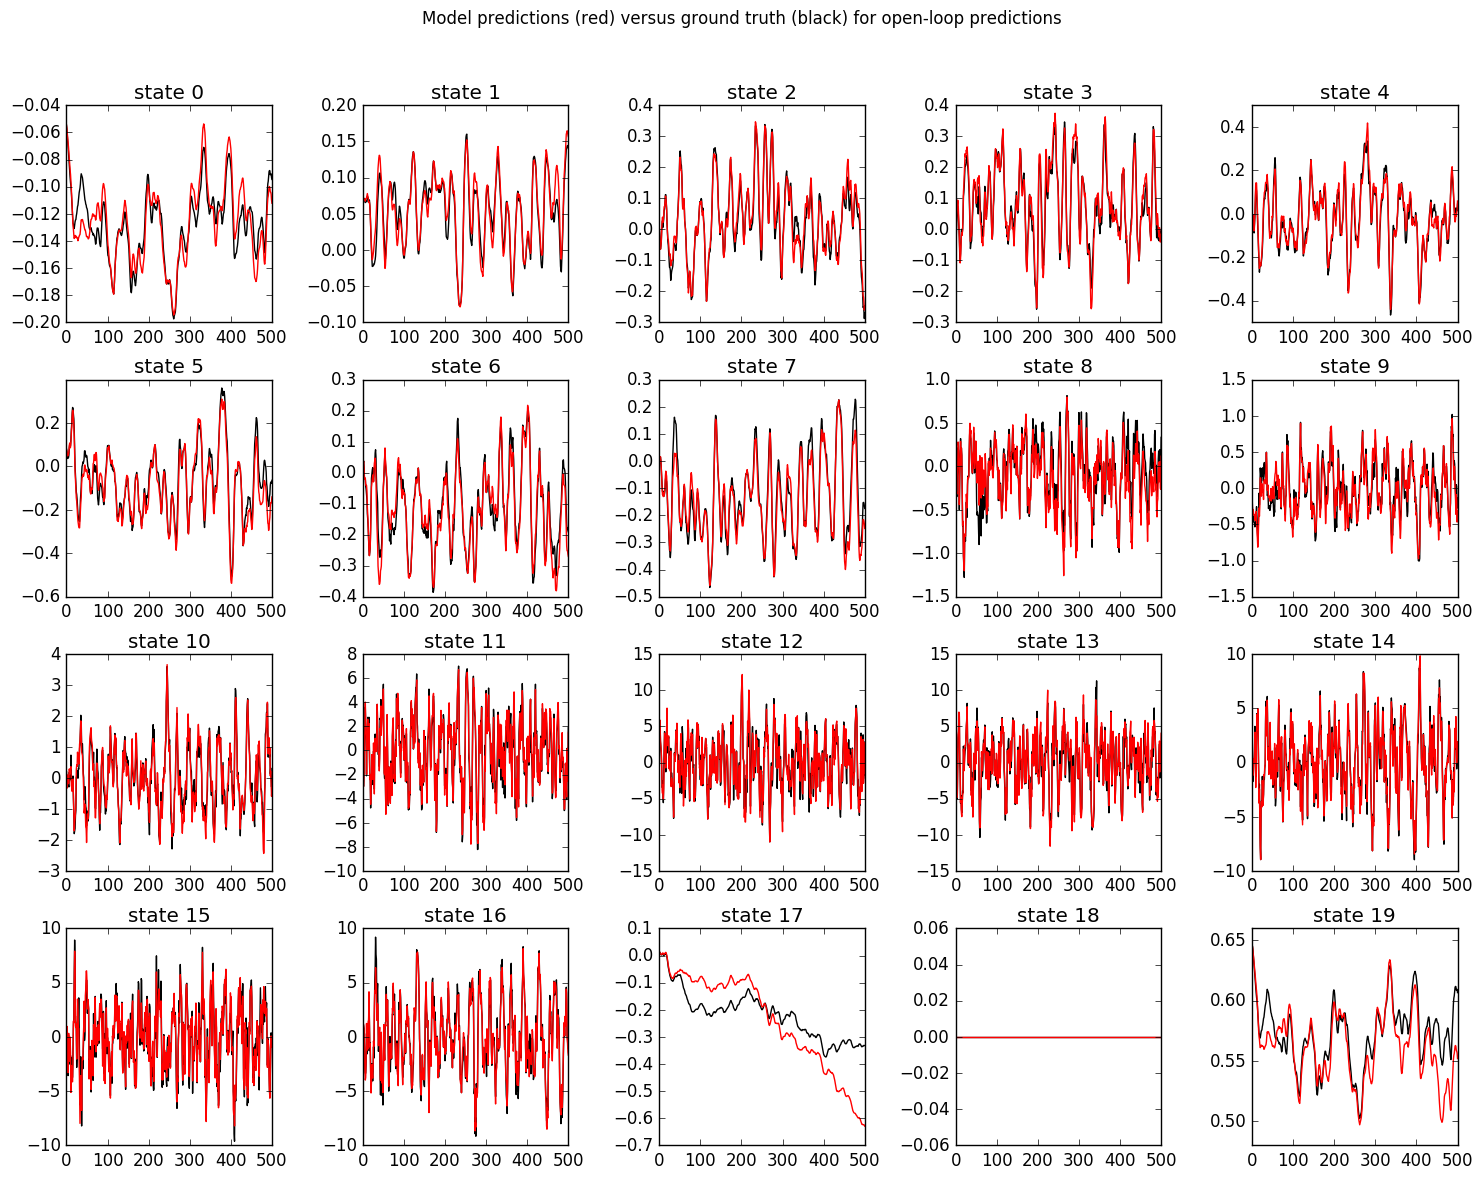
\includegraphics[width=1.0\textwidth]{prediction_009.png}
	 	\label{fig:q1}
	 	\caption[caption]{The plot of my most accurate dynamic model predictions.}
	\end{figure}

	\subsection{For which state dimension are the predictions the most inaccurate? Give a possible reason why the predictions are inaccurate.}
	The predictions of 17th dimension (state 17) is the most inaccurate.  It might be because state 17 rarely changes during random actions.  Therefore, the fitted model has not seen changes in state 17 and overfits.  It should also have something to do with the instability of open loop control.
	
	\pagebreak
	
	\section{Problem 2}
	\begin{center}
	\begin{tabular}{|c|c|c|}
		\hline
		          & \fontsize{20}{24} \selectfont  ReturnAvg & \fontsize{20}{24} \selectfont ReturnStd \\
		          \hline
	\fontsize{20}{24} \selectfont Random Policy & \fontsize{20}{24} \selectfont -156.836  &   \fontsize{20}{24} \selectfont 44.0595 \\
	\hline
	\fontsize{20}{24} \selectfont model-based controller (MPC) & \fontsize{20}{24} \selectfont 13.0374  &   \fontsize{20}{24} \selectfont 29.8065 \\
	\hline
	\end{tabular}
	\end{center}
	\hfill \linebreak
	\begin{lstlisting}
		10-19 09:19:30 HalfCheetah_q2_19-10-2018_09-19-30 INFO     Gathering random dataset
		10-19 09:19:31 HalfCheetah_q2_19-10-2018_09-19-30 INFO     Creating policy
		10-19 09:19:38 HalfCheetah_q2_19-10-2018_09-19-30 INFO     Random policy
		10-19 09:19:38 HalfCheetah_q2_19-10-2018_09-19-30 INFO     ---------  ---------
		10-19 09:19:38 HalfCheetah_q2_19-10-2018_09-19-30 INFO     ReturnAvg  -156.836
		10-19 09:19:38 HalfCheetah_q2_19-10-2018_09-19-30 INFO     ReturnMax   -92.4933
		10-19 09:19:38 HalfCheetah_q2_19-10-2018_09-19-30 INFO     ReturnMin  -251.131
		10-19 09:19:38 HalfCheetah_q2_19-10-2018_09-19-30 INFO     ReturnStd    44.0595
		10-19 09:19:38 HalfCheetah_q2_19-10-2018_09-19-30 INFO     ---------  ---------
		10-19 09:19:38 HalfCheetah_q2_19-10-2018_09-19-30 DEBUG    
		10-19 09:19:38 HalfCheetah_q2_19-10-2018_09-19-30 DEBUG    : total      0.0 (0.0%)
		10-19 09:19:38 HalfCheetah_q2_19-10-2018_09-19-30 DEBUG    : other      0.0 (0.0%)
		10-19 09:19:38 HalfCheetah_q2_19-10-2018_09-19-30 DEBUG    
		10-19 09:19:38 HalfCheetah_q2_19-10-2018_09-19-30 INFO     Training policy....
		10-19 09:19:41 HalfCheetah_q2_19-10-2018_09-19-30 INFO     Evaluating policy...
		10-19 09:26:37 HalfCheetah_q2_19-10-2018_09-19-30 INFO     Trained policy
		10-19 09:26:37 HalfCheetah_q2_19-10-2018_09-19-30 INFO     -----------------  -----------
		10-19 09:26:37 HalfCheetah_q2_19-10-2018_09-19-30 INFO     ReturnAvg           13.0374
		10-19 09:26:37 HalfCheetah_q2_19-10-2018_09-19-30 INFO     ReturnMax           53.6981
		10-19 09:26:37 HalfCheetah_q2_19-10-2018_09-19-30 INFO     ReturnMin          -32.5848
		10-19 09:26:37 HalfCheetah_q2_19-10-2018_09-19-30 INFO     ReturnStd           29.8065
		10-19 09:26:37 HalfCheetah_q2_19-10-2018_09-19-30 INFO     TrainingLossFinal    0.0275348
		10-19 09:26:37 HalfCheetah_q2_19-10-2018_09-19-30 INFO     TrainingLossStart    0.999107
		10-19 09:26:37 HalfCheetah_q2_19-10-2018_09-19-30 INFO     -----------------  -----------
		10-19 09:26:37 HalfCheetah_q2_19-10-2018_09-19-30 DEBUG    
		10-19 09:26:37 HalfCheetah_q2_19-10-2018_09-19-30 DEBUG    : total      419.0 (100.0%)
		10-19 09:26:37 HalfCheetah_q2_19-10-2018_09-19-30 DEBUG    : get action 414.5 (98.9%)
		10-19 09:26:37 HalfCheetah_q2_19-10-2018_09-19-30 DEBUG    : train policy 3.3 (0.8%)
		10-19 09:26:37 HalfCheetah_q2_19-10-2018_09-19-30 DEBUG    : env step   0.7 (0.2%)
		10-19 09:26:37 HalfCheetah_q2_19-10-2018_09-19-30 DEBUG    : other      0.6 (0.1%)
		10-19 09:26:37 HalfCheetah_q2_19-10-2018_09-19-30 DEBUG    
		
	\end{lstlisting}
	
	\pagebreak
	
	\section{Problem 3a}
	\begin{figure}[!htbp] 
		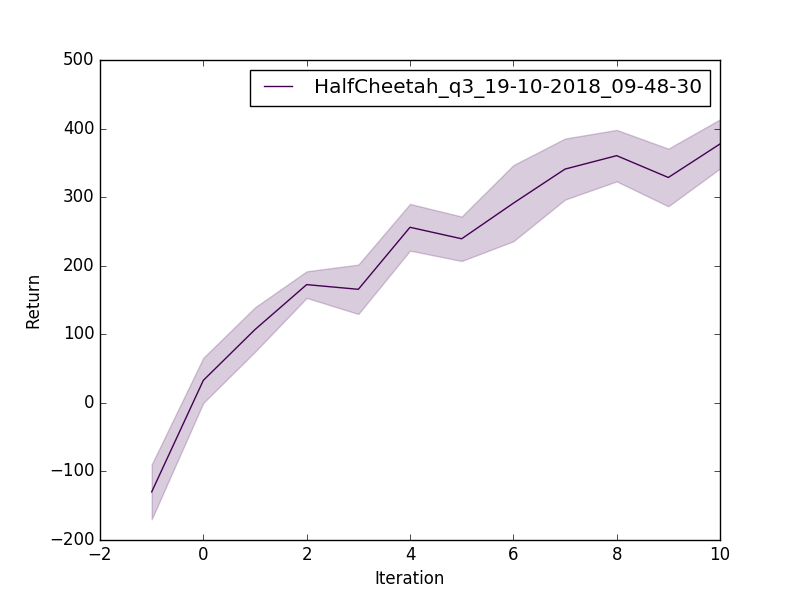
\includegraphics[width=0.6\textwidth]{question3a.png}
		\caption[caption]{
			The returns versus iteration of model-based controller (MPC).
		}\label{fig:q3a}
	\end{figure}

  \pagebreak
	
  \section{Problem 3b}
  \begin{figure}[!htbp]
  	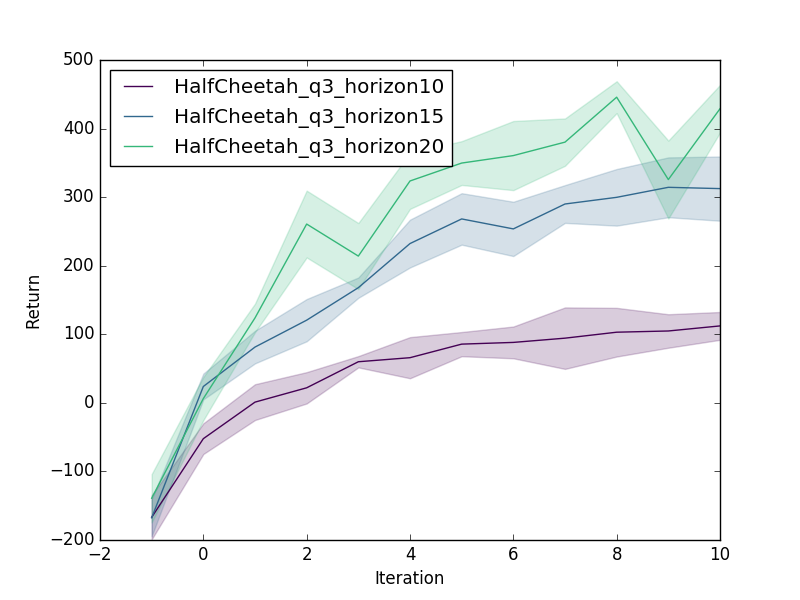
\includegraphics[width=0.48\textwidth]{HalfCheetah_q3_mpc_horizon.png}
  	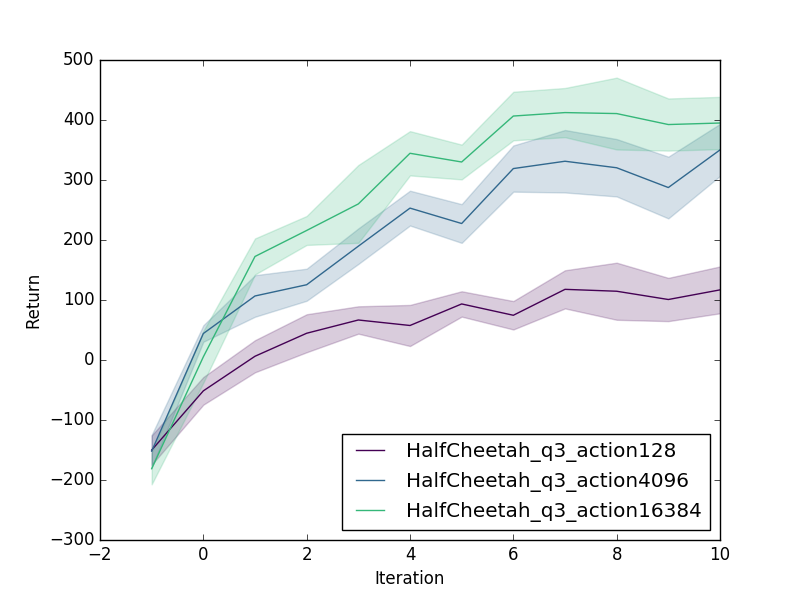
\includegraphics[width=0.48\textwidth]{HalfCheetah_q3_actions.png}
  	\floatbox[{\capbeside\thisfloatsetup{capbesideposition={right,center},capbesidewidth=0.48\textwidth}}]{figure}[\FBwidth]
  	{\caption[caption]{
  		Comparing performance when varying hyperparameters. \\ \hspace{0.4\textwidth}
  		Top left: MPC horizon; \\ \hspace{0.4\textwidth}
  		Top Right: the number of randomly sampled action sequences used for planning; \\ \hspace{0.4\textwidth}
  		Bottom right: the number of neural network layers for the learned dynamics model.
  		}}
  	{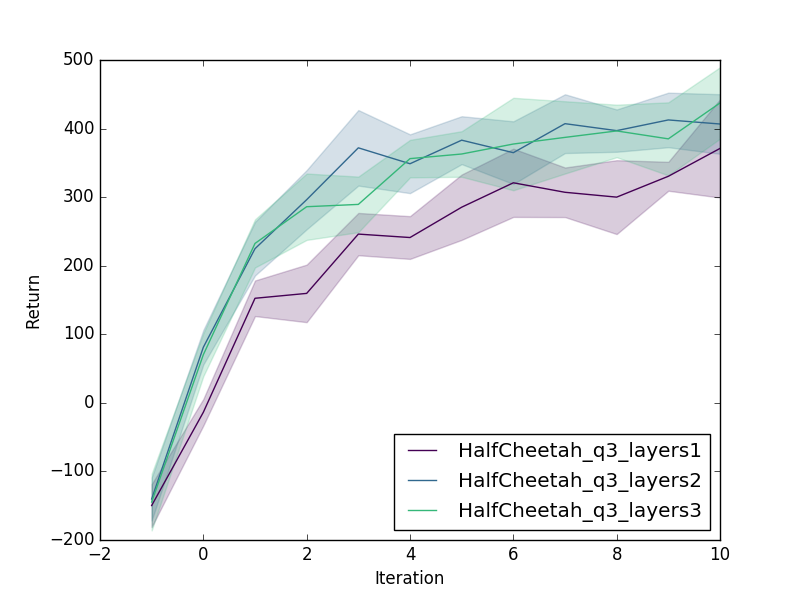
\includegraphics[width=0.48\textwidth]{HalfCheetah_q3_nn_layers.png}}
  	\label{fig:q3b}
  \end{figure}

  \pagebreak
  \section{bonus}
  \textit{Instead of performing action selection using random action sequences, use
  	the Cross Entropy Method (CEM). (See pseudo-code on Wikipedia.) How
  	much does CEM improve performance?}
  
  In my result, the cross entropy method doesn't improve the result at all.  I think is because the action space is small enough and our number of sample actions is large enough.  This makes uniform sampling enough to cover most of the action space and gives good results.\\
  At later iterations, CEM overfits to the original low cost region which makes it harder to find new low cost regions.
  
  \begin{figure}[!htbp]
  	\floatbox[{\capbeside\thisfloatsetup{capbesideposition={right,center},capbesidewidth=0.4\textwidth}}]{figure}[\FBwidth]
  	{\caption[caption]{
  			Comparing performance of random sampling and cross entropy method. \\ \hspace{0.4\textwidth}
  			Violet: random sampling; \\ \hspace{0.4\textwidth}
  			Cyan: cross entropy method (CEM)
  	}\label{fig:bonus3}}
  	{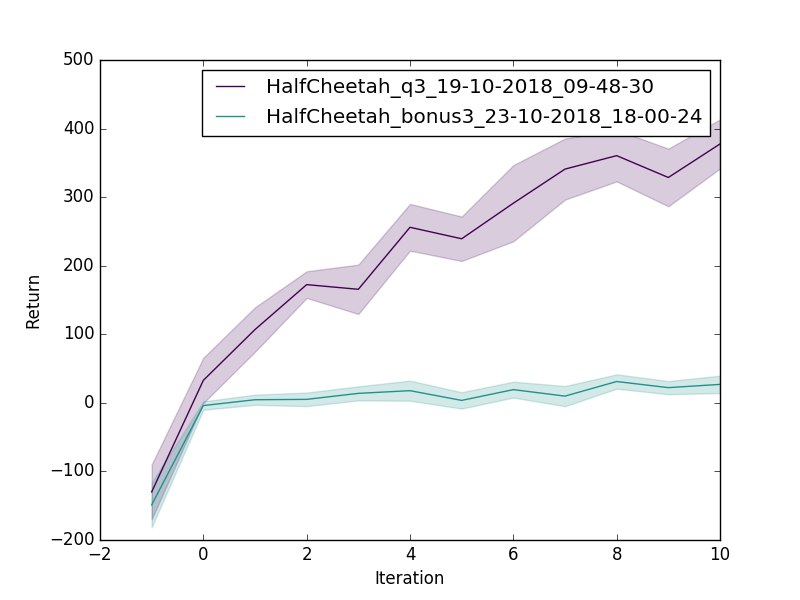
\includegraphics[width=0.48\textwidth]{bonus3.png}}
  \end{figure}
  
  
  \begin{lstlisting}
  10-20 17:35:50 HalfCheetah_q2_bonus INFO     Gathering random dataset
  10-20 17:35:51 HalfCheetah_q2_bonus INFO     Creating policy
  10-20 17:36:14 HalfCheetah_q2_bonus INFO     Random policy
  10-20 17:36:14 HalfCheetah_q2_bonus INFO     ---------  --------
  10-20 17:36:14 HalfCheetah_q2_bonus INFO     ReturnAvg  -147.093
  10-20 17:36:14 HalfCheetah_q2_bonus INFO     ReturnMax  -102.979
  10-20 17:36:14 HalfCheetah_q2_bonus INFO     ReturnMin  -186.081
  10-20 17:36:14 HalfCheetah_q2_bonus INFO     ReturnStd    27.542
  10-20 17:36:14 HalfCheetah_q2_bonus INFO     ---------  --------
  10-20 17:36:14 HalfCheetah_q2_bonus DEBUG    
  10-20 17:36:14 HalfCheetah_q2_bonus DEBUG    : total      0.0 (100.0%)
  10-20 17:36:14 HalfCheetah_q2_bonus DEBUG    : other      0.0 (100.0%)
  10-20 17:36:14 HalfCheetah_q2_bonus DEBUG    
  10-20 17:36:14 HalfCheetah_q2_bonus INFO     Training policy....
  10-20 17:36:16 HalfCheetah_q2_bonus INFO     Evaluating policy...
  10-20 17:54:08 HalfCheetah_q2_bonus INFO     Trained policy
  10-20 17:54:08 HalfCheetah_q2_bonus INFO     -----------------  -----------
  10-20 17:54:08 HalfCheetah_q2_bonus INFO     ReturnAvg          -11.5704
  10-20 17:54:08 HalfCheetah_q2_bonus INFO     ReturnMax           18.5725
  10-20 17:54:08 HalfCheetah_q2_bonus INFO     ReturnMin          -31.9431
  10-20 17:54:08 HalfCheetah_q2_bonus INFO     ReturnStd           13.4393
  10-20 17:54:08 HalfCheetah_q2_bonus INFO     TrainingLossFinal    0.0298326
  10-20 17:54:08 HalfCheetah_q2_bonus INFO     TrainingLossStart    1.04421
  10-20 17:54:08 HalfCheetah_q2_bonus INFO     -----------------  -----------
  10-20 17:54:08 HalfCheetah_q2_bonus DEBUG    
  10-20 17:54:08 HalfCheetah_q2_bonus DEBUG    : total      1074.8 (100.0%)
  10-20 17:54:08 HalfCheetah_q2_bonus DEBUG    : get action 1070.9 (99.6%)
  10-20 17:54:08 HalfCheetah_q2_bonus DEBUG    : train policy 2.7 (0.3%)
  10-20 17:54:08 HalfCheetah_q2_bonus DEBUG    : env step   0.8 (0.1%)
  10-20 17:54:08 HalfCheetah_q2_bonus DEBUG    : other      0.3 (0.0%)
  10-20 17:54:08 HalfCheetah_q2_bonus DEBUG    
  
  \end{lstlisting}
  
	
\end{document}